%% An Introduction to LaTeX Thesis Template of Wuhan University
%%
%% Created by WHUTUG

%\documentclass[oneside,type=master]{whu-thesis}
\documentclass[type=master]{whu-thesis}
%%% 去掉空白页,在打印时删除 %%%
\renewcommand{\cleardoublepage}{\clearpage}
%%% 去掉空白页,在打印时删除 %%%
\usepackage{enumitem}
\usepackage{titlesec}
\usepackage{titletoc}
\usepackage{amsfonts}
\usepackage{ulem}
\usepackage{zhnumber}
\usepackage{pdfpages}
\usepackage{setspace}
\usepackage{ragged2e}

%%% 如果需要使用\mathbb数学字体(比如期望,KL散度,示性函数等),
%%% 请使用\mathbbalt命令以使其正确渲染。

\newcommand{\upcite}[1]{\textsuperscript{\cite{#1}}} 
\renewcommand{\theequation}{\arabic{chapter}-\arabic{equation}}


\renewcommand{\thetable}{\arabic{chapter}-\arabic{table}}
\renewcommand{\thefigure}{\arabic{chapter}-\arabic{figure}}

\whusetup
  {
    info               =
      {
        title          = {论\ \ 文\ \ 题\ \ 目},
        title*         = {Research on ××××××××××××},
        student-number = {2010201020009},
        school         = {院系名称},
        author         = {张三},
        author*        = {Zhang San},
        major          = {摄影测量与遥感},
        advisor        = {李某 , 副教授},
        advisor*       = {Prof. , Li Mou},
        direction      = {计算机视觉},        
        subject        = {学科},
        date           = {2022/5},
        date*          = {May, 2022},
        school*        = {School of Remote Sensing and Information Engineering},
        keywords       = {计量学, 时基误差, 宽带取样示波器},
        keywords*      = {metrolog, time base error, broadband sampling oscilloscope},
      },
    style              =
      {
        graphics-path  = {{figures/}{data/}},
        bib-style      = numerical
        % list-of-figures,
        % list-of-tables,
      },
    element            =
      {
        abstract       = {pages/abstract},
        abstract*      = {pages/enabstract},
        bibliography   = {ref/refs , ref/thu},
        achievements   = {pages/achievements},
        projects       = {pages/projects},
        authorization  = {pages/authorization_blind.pdf},
        %appendix       = {pages/appendix},
        thanks         = {pages/thanks},
        %innovation     = {pages/innovation.pdf},
      }
  }

\begin{document}
  
%%----------- 主体部分 ----------- %%
%在生成摘要后,重新将chapter定义为2号字
% Chapter 1

\chapter{绪论}

\label{sec:ch1}

\section{研究背景与意义}

随着人类社会的发展,尤其是近年来城市化、现代化进程的迅速推进,大量人口集中向城市流动,并集中活动于各个机场、车站、体育馆、商场、写字楼等室内公共环境已成为现代社会生活的常态。在这些人员高度密集的室内场所中,发生火灾、踩踏等公共安全事故的潜在威胁也越来越大。

\section{国内外研究进展}

在过去几十年中,行人疏散被认为是具有社会意义的研究对象。在计算机得到普及之前,早期行人疏散的研究方法主要分为三种:1. 典型事故案例研究;2. 真实实验研究;3. 调查问卷。其中,事故案例研究属于被动式的吸取教训,有助于初步掌握疏散逃生的基本原则,但由于留下完整记录的事故案例非常稀少,这种研究方式难以深入探寻背后的原理。

\subsection{行人疏散动力学}

\subsubsection{行人疏散动力学}

早期行人疏散研究,主要是第二次工业革命后,由第一批进行城市化的先发发达国家基于自身需要进行研究。美国在该研究方向的起源非常早。早在20 世纪初,美国就已经开始在车站、商场、剧院、办公楼等公共场所进行行人运动的观测、演习和实验,总结了许多人员疏散的经验和客观规律 \\ 

{\color{red}正文第一章必须处于右边,页码从1开始编码。正文中间不要出现空白页。正文是学位论文的核心部分,每一章都必须另页开始,即每一章都另起一页。

内容一律用宋体小四号字(英文或数字用Times New Roman格式),行间距设置为最小值20磅,两端对齐,首行缩进2字符,各章、节应有序号。

一级标题黑体二号加粗,单倍行距,段前段后各12磅,居中

二级标题黑体三号加粗,单倍行距,段前段后各12磅,左对齐

三级标题宋体小三加粗,单倍行距,段前段后各12磅,左对齐

四级标题(如果需要的话)宋体小四加粗,单倍行距,段前段后各12磅,左对齐}

\newpage

“不确定性”这个概念与1927 年由德国物理学家海森堡首次提出,用来描绘微观世界中,一个微观粒子的位置和动量无法被同时准确观测到的现象,即:
\begin{equation}
\setlength\abovedisplayskip{6pt} % 6=12号字体/2
\setlength\belowdisplayskip{6pt} % 6=12号字体/2
\label{eq:ch1_1}
G=\{I ; S ; \Pi i(s)\}    
\end{equation}
{\color{red}公式格式:按照章节采用(1-1)的格式进行编号,置于公式同一行的右边,楷体小四加粗,段前段后各0.5行,右对齐。} \\

本次实验的来源主要来自浙江省测绘局地理信息局和浙江省统计局网站。变量值如表1-1所示。


\begin{table}[h]
\renewcommand{\arraystretch}{1.5}
\centering
\caption{浙江省地理信息从业人员比重(单位:\%)}
\begin{tabular}{ccccc}
\toprule
\makebox[0.15\textwidth][c]{\textbf{地点}} & \makebox[0.15\textwidth][c]{\textbf{2011年}} & \makebox[0.15\textwidth][c]{\textbf{2012年}} & \makebox[0.15\textwidth][c]{\textbf{2013年}} & \makebox[0.15\textwidth][c]{\textbf{2014年}} \\
\midrule
杭州 & 29.31 & 31.46 & 30.49 & 28.77 \\
宁波 & 28.55 & 29.34 & 30.67 & 35.61 \\
温州 & 24.81 & 29.44 & 28.97 & 39.69 \\
嘉兴 & 33.97 & 36.23 & 40.63 & 32.38 \\
金华 & 32.14 & 31.94 & 32.14 & 33.00 \\
丽水 & 35.54 & 34.89 & 35.00 & 35.93 \\
\bottomrule
\end{tabular}
\label{tab:ch1_1}
\flushleft
\justifying {\kaishu \bfseries \small {\qquad 说明:2011-2014年浙江省各地市具有高级和中级技术职称的地理信息从业人员数量占本市地理信息从业人员总数的比重}}
\end{table}


{\color{red}表格格式:表格居中,表格标题置于表格上方居中,楷体五号加粗,单倍行距,段前0.5行,段后0.5行。编号根据每一个章节,按照“表1-1”的格式进行编号。表格内容采用宋体五号字。如果有说明文字,放在表格下方,楷体五号加粗,单倍行距,段前0.5行,段后0.5行,首行空两个字符

一般要防止出现表格跨页的情况,如果表格实在太大,无法放在一页中可以采用续表的形式。如表格不止2页,可用续表1,续表2}

\newpage

\begin{figure}[h]
\centering
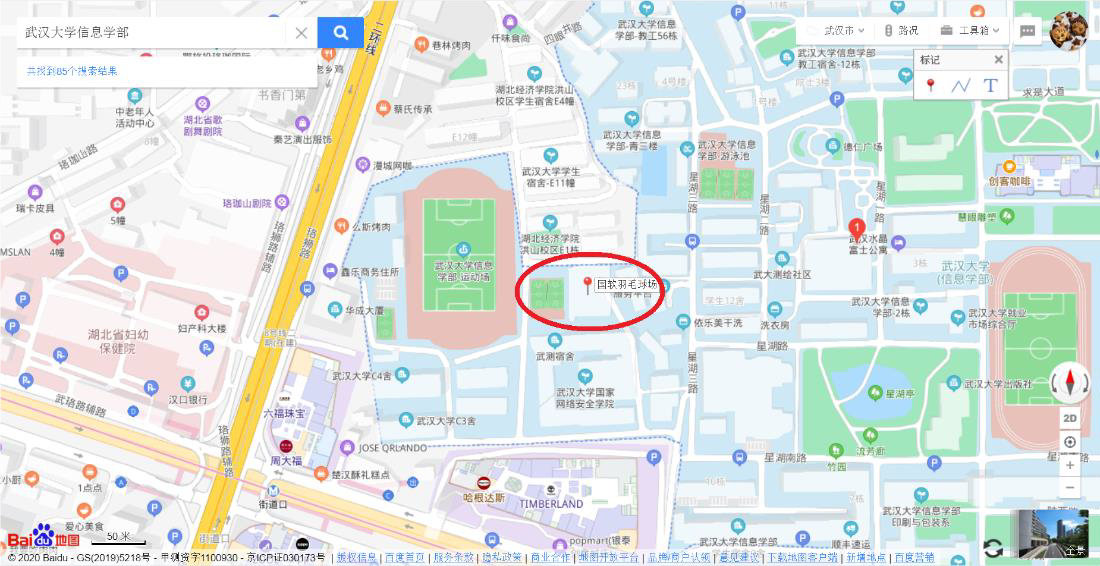
\includegraphics[width=0.85\textwidth]{figures/fig1.png}
\caption{真人实验场地}
\label{fig:ch1_1}
\flushleft
\justifying {\kaishu \bfseries \small {\qquad 说明:2011-2014年浙江省各地市具有高级和中级技术职称的地理信息从业人员数量占本市地理信息从业人员总数的比重}}
\end{figure}

{\color{red}图格式:图片居中,图标题置于图下方居中,楷体五号加粗,单倍行距,段后0.5行,段前0.5行。编号根据每一个章节,按照“图1-1”的格式进行编号。如果有说明文字,放在图名下方,楷体五号加粗,单倍行距,段前0.5行,段后0.5行,首行缩进字符。}
% \include{pages/chapter2}
% \include{pages/chapter3}
% \include{pages/chapter4}
% \include{pages/chapter5}

\nocite{*} %显示所有文献,请注释!!!
\end{document}
